\documentclass{article}
\usepackage{fullpage}

%load needed packages
\usepackage{graphicx}
\usepackage{subcaption}
\usepackage{array}
\usepackage{booktabs}
\usepackage[utf8]{inputenc}
\usepackage[T1]{fontenc}
\usepackage{url}
\usepackage[spanish]{babel} % Paquete para el idioma español
\usepackage{float}  % Necesario para [H]
\usepackage{listings}
\usepackage{xcolor}

\definecolor{codegreen}{HTML}{5AB2FF}
\definecolor{morado}{HTML}{AD88C6}
\definecolor{BG}{HTML}{EEEEEE}
\definecolor{azul}{HTML}{4D869C}
\definecolor{sqlblue}{HTML}{FF8C00} % Color para las palabras clave SQL

% Estilo para DDL
\lstdefinestyle{ddlstyle}{
	language=SQL,
	backgroundcolor=\color{BG},
	commentstyle=\color{codegreen},
	basicstyle=\ttfamily\small,
	keywordstyle=\color{azul},
	stringstyle=\color{morado},
	showstringspaces=false,
	breaklines=true,
	frame=shadowbox,
	numbers=left,
	numberstyle=\tiny\color{gray},
	captionpos=b,
}

% Estilo para SQL
\lstdefinestyle{sqlstyle}{
	language=SQL,
	backgroundcolor=\color{BG},
	commentstyle=\color{codegreen},
	basicstyle=\ttfamily\small,
	keywordstyle=\color{sqlblue}, % Color diferente para palabras clave SQL
	stringstyle=\color{morado},
	showstringspaces=false,
	breaklines=true,
	frame=shadowbox,
	numbers=left,
	numberstyle=\tiny\color{gray},
	captionpos=b,
}

\begin{document}
	
	
	
	% Portada
	\begin{titlepage}
		\centering
		\vspace*{3cm}
		
		% Título destacado
		{\Huge \textbf{Análisis de datos y reporte con PowerBI}\\[0.5cm]}
		
		% Espacio y logotipo (si lo tienes, por ejemplo el logo de tu universidad)
		\vspace{2cm}
		
\includegraphics[width=0.3\textwidth]{images/uma_logo.jpg}\\[1cm]
		
		% Nombre del autor
		{\LARGE \textbf{Alejandro Silva Rodríguez}\\[0.5cm]}

		{\large \textit{Almacenes De Datos}\\
			Universidad de Málaga\\
		}
		
		\vfill
		
		% Fecha en la parte inferior de la página
		{\large Diciembre 2024}
	\end{titlepage}
	
	% indice
	\tableofcontents
	
	\newpage
\section{Introducción}
\label{sec:introduccion}

En el contexto hospitalario actual, el análisis avanzado de datos se ha convertido en una herramienta indispensable para optimizar la toma de decisiones y mejorar la gestión de recursos en áreas críticas como las Unidades de Cuidados Intensivos (UCI). El análisis detallado del gasto en medicamentos, que representa una proporción significativa de los costos operativos, requiere técnicas especializadas que permitan explorar grandes volúmenes de datos desde múltiples perspectivas.\\

Tras la construcción de un almacén de datos orientado al análisis del gasto en medicamentos y la implementación de estructuras que soportan consultas analíticas avanzadas, el siguiente paso lógico es realizar un análisis exhaustivo del cubo multidimensional y generar reportes estadísticos. Este trabajo se enfoca en el desarrollo de un dashboard interactivo para analizar el gasto en medicamentos en pacientes ingresados en UCI en hospitales de EE.UU. \cite{eicu_crd}.


\section{Objetivos}


El objetivo principal de esta tarea es diseñar y documentar un dashboard interactivo utilizando el almacén de datos del proyecto.

\begin{itemize}
	\item Utilizar el almacén de datos del proyecto para generar un dashboard o informe interactivo que permita analizar los datos de forma visual y comprensible.

	\item Mostrar para cada gráfica, tabla o elemento del informe la consulta MDX que provee los datos utilizados, incluyendo el texto de la consulta y la validación de los resultados obtenidos.
	
\end{itemize}


\section{Dashboard}

\subsection{Preparación de los Datos}
Antes de comenzar a crear el dashboard, es necesario importar el origen de datos seleccionando la opción \textit{Analysis Services} (Figura \ref{fig:origen}). Para manejar los datos, se pueden adoptar dos enfoques: trabajar con ellos en modo directo (consultándolos conforme se necesitan) o importarlos al proyecto. Es fundamental considerar que, si la cantidad de datos es muy grande, el modo directo podría afectar negativamente el rendimiento.

\begin{figure}[H]
	\centering
	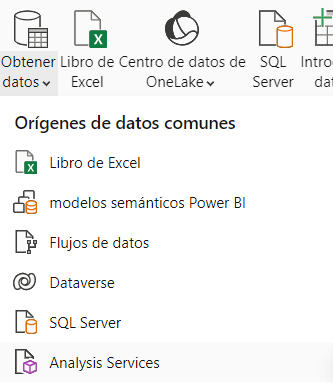
\includegraphics[width=.3\textwidth]{images/origen_datos.png}
	\caption{Selección del Origen de Datos.}
	\label{fig:origen}
\end{figure}

\subsection{Creación del Dashboard}

\subsubsection{Diseño General}
Organizamos el diseño general del dashboard disponiendo formas para demarcar las áreas destinadas a controles similares. Posteriormente, procedemos a insertar las visualizaciones correspondientes (Figura \ref{fig:visualizaciones}).

\begin{figure}[H]
	\centering
	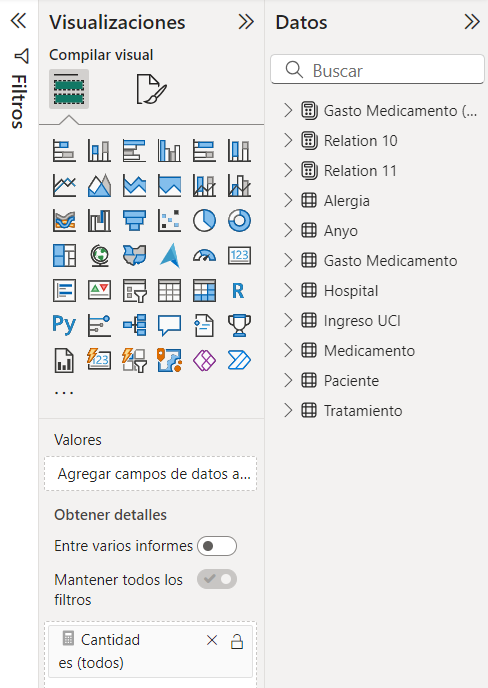
\includegraphics[width=.4\textwidth]{images/graficas.png}
	\caption{Inserción de Visualizaciones.}
	\label{fig:visualizaciones}
\end{figure}

\subsubsection{Tarjetas Resumen}
\begin{itemize}
	\item Insertamos dos \textbf{tarjetas} para mostrar el volumen total de fluidos y la cantidad total de medicamentos utilizados.
	\item Personalizamos el estilo de las tarjetas modificando bordes, sombras y colores.
\end{itemize}

\subsubsection{Visualizaciones}
Diseñamos visualizaciones que aporten valor analítico, incluyendo entre otros:
\begin{itemize}
	\item Cantidad de medicamento consumido por región, fuente de admisión y tratamiento, para predecir gastos futuros.
	\item Relación entre el número de camas y el volumen de medicamentos necesarios, para estimar la cantidad a adquirir según el tamaño del hospital.
	\item Volumen de fluidos utilizado por año y tipo de unidad, para anticipar necesidades de capacidad.
	\item Gasto por hospital, con el objetivo de analizar los costos totales por institución.
\end{itemize}

\subsubsection{Filtros y Segmentaciones}
En el lado izquierdo del dashboard:
\begin{itemize}
	\item Incorporamos segmentaciones para \textbf{Año}, \textbf{Estado de Alta}, \textbf{Número de Camas} y \textbf{Tipo de Unidad}.
\end{itemize}

\subsection{Formato y Estilo}
Para otorgar un acabado profesional al dashboard:
\begin{enumerate}
	\item Modificamos el fondo del lienzo desde \textbf{Formato de página} > \textbf{Fondo}, utilizando una imagen de gradiente previamente diseñada.
	\item Ajustamos los colores seleccionando un tema en el apartado \textbf{Ver} (Figura \ref{fig:temas}).
\end{enumerate}

\begin{figure}[H]
	\centering
	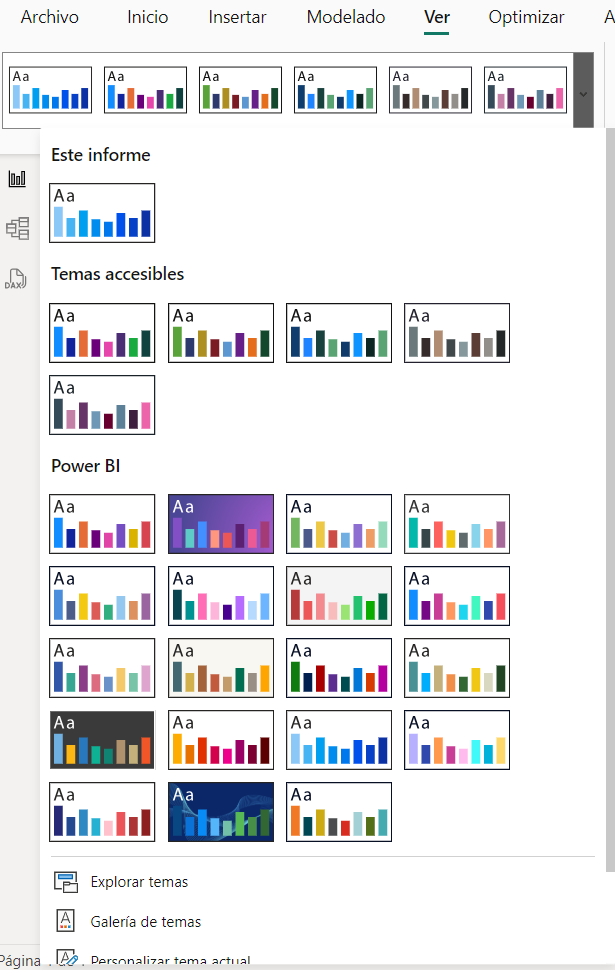
\includegraphics[width=.3\textwidth]{images/temas.png}
	\caption{Aplicación de Tema.}
	\label{fig:temas}
\end{figure}

Finalmente, obtenemos el dashboard terminado (Figura \ref{fig:dashboard}).

\begin{figure}[H]
	\centering
	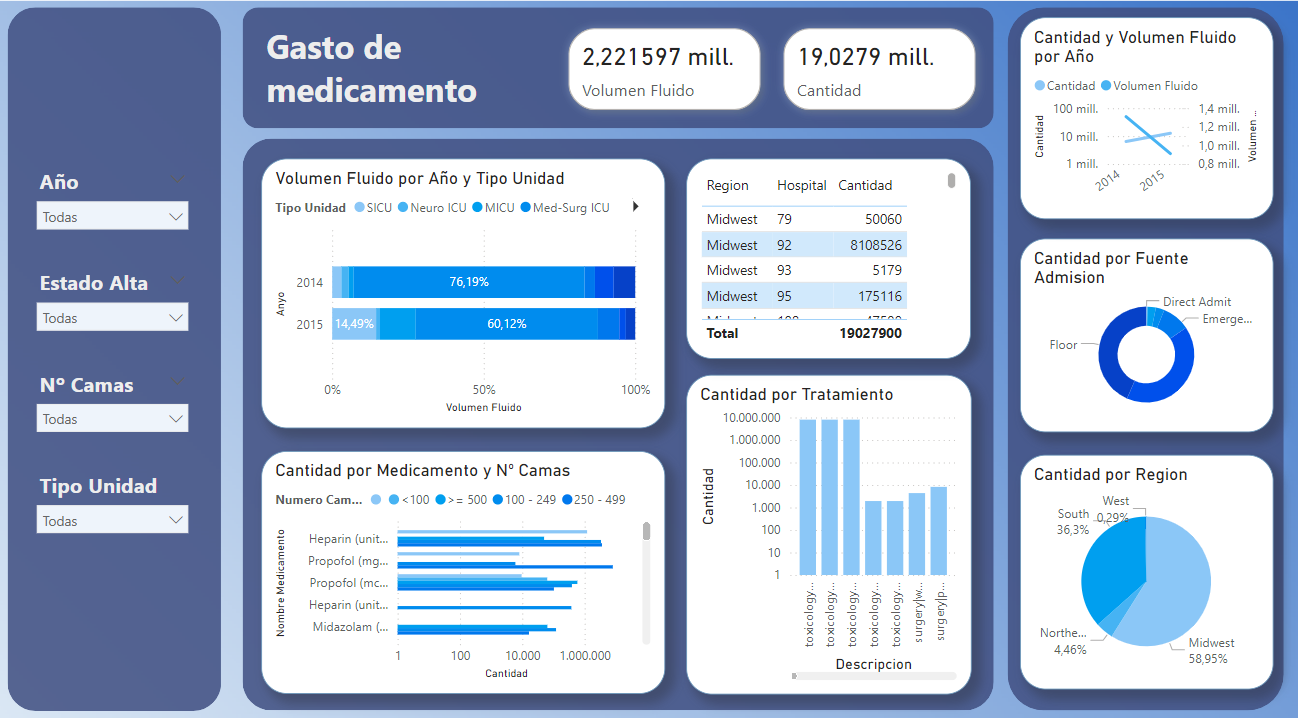
\includegraphics[width=\textwidth]{images/dashboard.png}
	\caption{Dashboard Finalizado.}
	\label{fig:dashboard}
\end{figure}


\section{Comprobación con consultas MDX}

Con el objetivo de verificar que las visualizaciones son fieles a los datos, por cada una se hará una consulta MDX para comprobar que los valores son similares.\\

En la figura \ref{fig:fuente_admision_comparacion} se observa el gráfico de cantidad de gasto de medicamento por fuente de admision, Tanto en la visualización como en la consulta se observa como Floor tiene el mayor porcentaje (43\%) y desconocido tiene un porcentaje bastante grande (41\%)
\begin{figure}[H]
	\centering
	\begin{subfigure}[b]{0.4\textwidth}
		\centering
		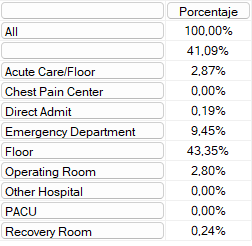
\includegraphics[width=\textwidth]{images/cantidad_fuente_admision_mdx.png}
		\caption{Cantidad por fuente de admisión (MDX).}
		\label{fig:fuente_admision_mdx}
	\end{subfigure}
	\hfill
	\begin{subfigure}[b]{0.4\textwidth}
		\centering
		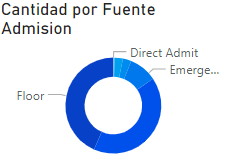
\includegraphics[width=\textwidth]{images/cantidad_fuente_admision_pbx.png}
		\caption{Cantidad por fuente de admisión (PBX).}
		\label{fig:fuente_admision_pbx}
	\end{subfigure}
	\caption{Comparación de la cantidad por fuente de admisión en consulta y gráfica.}
	\label{fig:fuente_admision_comparacion}
\end{figure}

\begin{lstlisting}[style=ddlstyle, label=lst:consulta1, caption=Cantidad por fuente de admisión]
	WITH 
	MEMBER [Measures].[Porcentaje] AS
	IIF(
	IsEmpty([Measures].[Cantidad]),
	null,
	Format(
	([Measures].[Cantidad] / 
	(SUM([Ingreso UCI].[Fuente Admision].MEMBERS, [Measures].[Cantidad]))) * 200, 
	"0.00"
	) + "%"
	)
	SELECT 
	NON EMPTY [Ingreso UCI].[Fuente Admision].MEMBERS ON ROWS,
	[Measures].[Porcentaje] ON COLUMNS
	FROM UCIDW
\end{lstlisting}

En la figura \ref{fig:region_comparacion} se observa la cantidad de medicamento gastado por region, los porcentajes son exactamente los esperados.

\begin{figure}[H]
	\centering
	\begin{subfigure}[b]{0.4\textwidth}
		\centering
		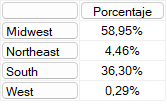
\includegraphics[width=\textwidth]{images/cantidad_region_mdx.png}
		\caption{Cantidad por región (MDX).}
		\label{fig:region_mdx}
	\end{subfigure}
	\hfill
	\begin{subfigure}[b]{0.4\textwidth}
		\centering
		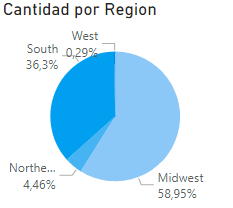
\includegraphics[width=\textwidth]{images/cantidad_region_pbx.png}
		\caption{Cantidad por región (PBX).}
		\label{fig:region_pbx}
	\end{subfigure}
	\caption{Comparación de la cantidad por región en consulta y gráfica.}
	\label{fig:region_comparacion}
\end{figure}

\begin{lstlisting}[style=ddlstyle, label=lst:consulta2, caption=Cantidad por Región]

WITH 
MEMBER [Measures].[Porcentaje] AS
IIF(
IsEmpty([Measures].[Cantidad]),
null,
Format(
([Measures].[Cantidad] / 
(SUM([Hospital].[Hospital].[Region].MEMBERS, [Measures].[Cantidad]))) * 100, 
"0.00"
) + "%"
)
SELECT 
NON EMPTY [Hospital].[Hospital].[Region].MEMBERS ON ROWS,
[Measures].[Porcentaje] ON COLUMNS
FROM UCIDW
\end{lstlisting}

En la figura \ref{fig:volumen_año_comparacion} se observa la cantidad y volumen de medicamento gastado por año. Los valores obtenidos en la consulta coninciden con la visualizacion.

\begin{figure}[H]
	\centering
	\begin{subfigure}[b]{0.4\textwidth}
		\centering
		\includegraphics[width=\textwidth]{images/cantidad_volumen_año_mdx.png}
		\caption{Cantidad y volumen por año (MDX).}
		\label{fig:volumen_año_mdx}
	\end{subfigure}
	\hfill
	\begin{subfigure}[b]{0.4\textwidth}
		\centering
		\includegraphics[width=\textwidth]{images/cantidad_volumen_año_pbx.png}
		\caption{Cantidad y volumen por año (PBX).}
		\label{fig:volumen_año_pbx}
	\end{subfigure}
	\caption{Comparación de la cantidad y volumen por año en consulta y gráfica.}
	\label{fig:volumen_año_comparacion}
\end{figure}

\begin{lstlisting}[style=ddlstyle, label=lst:consulta3, caption=Cantidad y Volumen por Año]

SELECT NON EMPTY[Anyo].[Jerarquia].[Anyo].MEMBERS ON ROWS, 
{[Measures].[Cantidad],[Measures].[Volumen Fluido]} ON COLUMNS
FROM UCIDW
\end{lstlisting}

En la figura \ref{fig:tratamiento_comparacion} se observa el gasto por tratamiento en escala logaritmica, es coherente la consulta con la visualización.
\begin{figure}[H]
	\centering
	\begin{subfigure}[b]{0.4\textwidth}
		\centering
		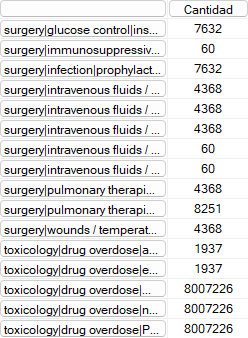
\includegraphics[width=\textwidth]{images/cantidad_tratamiento_mdx.png}
		\caption{Cantidad por tratamiento (MDX).}
		\label{fig:tratamiento_mdx}
	\end{subfigure}
	\hfill
	\begin{subfigure}[b]{0.4\textwidth}
		\centering
		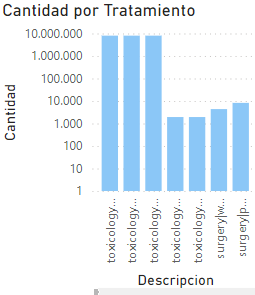
\includegraphics[width=\textwidth]{images/cantidad_tratamiento_pbx.png}
		\caption{Cantidad por tratamiento (PBX).}
		\label{fig:tratamiento_pbx}
	\end{subfigure}
	\caption{Comparación de la cantidad por tratamiento en consulta y gráfica.}
	\label{fig:tratamiento_comparacion}
\end{figure}

\begin{lstlisting}[style=ddlstyle, label=lst:consulta4, caption=Cantidad por Tratamiento]

SELECT NON EMPTY [Tratamiento].[Descripcion].MEMBERS ON ROWS, 
[Measures].[Cantidad] ON COLUMNS
FROM UCIDW
\end{lstlisting}

En la figura \ref{fig:region_hospital_comparacion} observamos una tabla con el gasto de medicamento en distintos hospitales, coincidiente con la consulta MDX.
\begin{figure}[H]
	\centering
	\begin{subfigure}[b]{0.2\textwidth}
		\centering
		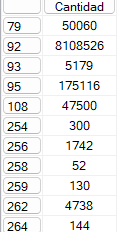
\includegraphics[width=\textwidth]{images/cantidad_region_hospital_tabla_mdx.png}
		\caption{Cantidad por región hospital (MDX).}
		\label{fig:region_hospital_mdx}
	\end{subfigure}
	\hfill
	\begin{subfigure}[b]{0.4\textwidth}
		\centering
		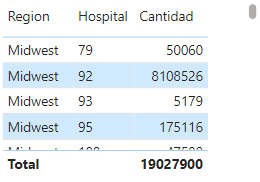
\includegraphics[width=\textwidth]{images/cantidad_region_hospital_tabla_pbx.png}
		\caption{Cantidad por región hospital (PBX).}
		\label{fig:region_hospital_pbx}
	\end{subfigure}
	\caption{Comparación de la cantidad por región hospital en consulta y gráfica.}
	\label{fig:region_hospital_comparacion}
\end{figure}

\begin{lstlisting}[style=ddlstyle, label=lst:consulta5, caption=Cantidad por Región y Hospital]

SELECT 
NON EMPTY  [Hospital].[Hospital].[Hospital].MEMBERS ON ROWS, 
[Measures].[Cantidad] ON COLUMNS
FROM UCIDW
\end{lstlisting}

En la figura \ref{fig:medicamento_camas_comparacion} se obserca el gasto por medicamento y numero de camas, que es coherente con la consulta MDX.
\begin{figure}[H]
	\centering
	\begin{subfigure}[b]{0.4\textwidth}
		\centering
		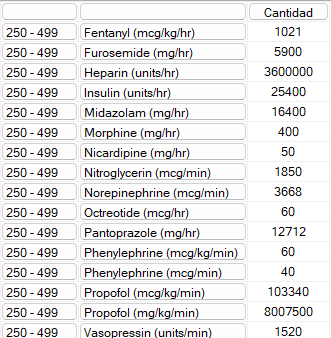
\includegraphics[width=\textwidth]{images/cantidad_medicamento_numero_camas_mdx.png}
		\caption{Cantidad por medicamento y número de camas (MDX).}
		\label{fig:medicamento_camas_mdx}
	\end{subfigure}
	\hfill
	\begin{subfigure}[b]{0.4\textwidth}
		\centering
		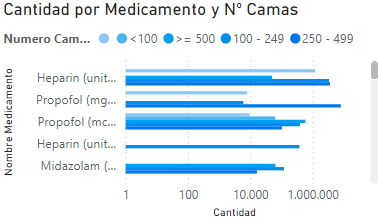
\includegraphics[width=\textwidth]{images/cantidad_medicamento_numero_camas_pbx.png}
		\caption{Cantidad por medicamento y número de camas (PBX).}
		\label{fig:medicamento_camas_pbx}
	\end{subfigure}
	\caption{Comparación de la cantidad por medicamento y número de camas en consulta y gráfica.}
	\label{fig:medicamento_camas_comparacion}
\end{figure}

\begin{lstlisting}[style=ddlstyle, label=lst:consulta6, caption=Cantidad por Medicamento y Número de Camas]

SELECT NON EMPTY [Hospital].[Numero Camas Categoria].MEMBERS * [Medicamento].[Nombre Medicamento].MEMBERS ON ROWS, 
[Measures].[Cantidad] ON COLUMNS
FROM UCIDW
\end{lstlisting}

En la figura \ref{fig:volumen_tipo_uci_comparacion} se observa el volumen de fluido por año portipo de unidad, estos valores parecen concordar con la consulta.
\begin{figure}[H]
	\centering
	\begin{subfigure}[b]{0.4\textwidth}
		\centering
		\includegraphics[width=\textwidth]{images/volumen_año_tipo_uci_mdx.png}
		\caption{Volumen por año y tipo de UCI (MDX).}
		\label{fig:volumen_tipo_uci_mdx}
	\end{subfigure}
	\hfill
	\begin{subfigure}[b]{0.4\textwidth}
		\centering
		\includegraphics[width=\textwidth]{images/volumen_año_tipo_uci_pbx.png}
		\caption{Volumen por año y tipo de UCI (PBX).}
		\label{fig:volumen_tipo_uci_pbx}
	\end{subfigure}
	\caption{Comparación del volumen por año y tipo de UCI en consulta y gráfica.}
	\label{fig:volumen_tipo_uci_comparacion}
\end{figure}

\begin{lstlisting}[style=ddlstyle, label=lst:consulta7, caption=Volúmen por Año y Tipo de UCI]

SELECT NON EMPTY [Anyo].[Jerarquia].CHILDREN * [Ingreso UCI].[Tipo Unidad].CHILDREN ON ROWS, 
[Measures].[Volumen Fluido] ON COLUMNS
FROM UCIDW

\end{lstlisting}


\section{Conclusiones}
\label{sec:conclusiones}

El uso de PowerBI para el diseño de dashboards interactivos ha facilitado una comprensión más detallada del gasto en medicamentos en las Unidades de Cuidados Intensivos (UCI). La validación de los datos a través de consultas MDX garantiza la fiabilidad de las visualizaciones generadas, lo que asegura una toma de decisiones más informada. Este enfoque demuestra cómo la combinación de herramientas de visualización y consultas analíticas puede optimizar el análisis de datos hospitalarios, mejorando la eficiencia en la gestión y el control de los recursos.


\section{Dificultades Encontradas}
	
Una de las principales dificultades que enfrenté fue aprender Power BI desde cero para poder crear algo relativamente complejo. Sin embargo, la curva de aprendizaje resultó ser bastante suave, ya que existen numerosos recursos, tutoriales y videos disponibles que facilitaron el proceso. Por otro lado, al importar los datos, me di cuenta de que intentar cargar el conjunto completo resultaba inviable debido al gran volumen de información. Aunque optar por un origen de datos directo para la publicación haría el proceso más sencillo, resulta más complejo y difícil de mantener a largo plazo. El desafío más significativo fue, sin duda, lograr que el dashboard realmente aportara valor en el proceso de toma de decisiones, ya que he tenido que intentar entender las necesidades y la complejidad de la administración del gasto de medicamento en un hospital.

	% Incluir la bibliografía
	\bibliographystyle{plain}  % Estilo de la bibliografía (por ejemplo, plain, alpha, ieee, etc.)
	\bibliography{bibli}  % Nombre del archivo .bib sin la extensión
	
\end{document}
